% ------------------------------------------------------------------------------
% TYPO3 CMS 8.3 - What's New - Chapter "In-Depth Changes" (Serbian Version)
%
% @author	Patrick Lobacher <patrick@lobacher.de> and Michael Schams <schams.net>
% @license	Creative Commons BY-NC-SA 3.0
% @link		http://typo3.org/download/release-notes/whats-new/
% @language	Serbian
% ------------------------------------------------------------------------------
% LTXE-CHAPTER-UID:		5ebcecbe-66abfa57-cf38bc00-aa637965
% LTXE-CHAPTER-NAME:	In-Depth Changes
% ------------------------------------------------------------------------------

\section{Korenite promene}
\begin{frame}[fragile]
	\frametitle{Korenite promene}

	\begin{center}\huge{Poglavlje 3:}\end{center}
	\begin{center}\huge{\color{typo3darkgrey}\textbf{Korenite promene}}\end{center}

\end{frame}

% ------------------------------------------------------------------------------
% LTXE-SLIDE-START
% LTXE-SLIDE-UID:		5384c02d-1618ead3-cd23b5b7-1ba7be5d
% LTXE-SLIDE-ORIGIN:	bd33b29d-c20d1765-f923f78e-43bfb0bf English
% LTXE-SLIDE-TITLE:		Feature #74365: Add Linkservice for Unified Referencing Syntax (1)
% LTXE-SLIDE-REFERENCE:	Feature-74365-LinkServiceForUnifiedReferencingSyntax.rst
% ------------------------------------------------------------------------------
\begin{frame}[fragile]
	\frametitle{Korenite promene}
	\framesubtitle{Dodat je Linkservice za jedinstvenu sintaksu referenci (1)}

	\begin{itemize}

		\item Sredstva koja su se koristila unutar TYPO3 u proslosti su bila referencirana koristeci 
			vise razlicitih sintaksnih formi.

		\item TYPO3 sada podrzava moderne nacine referenciranja sredstava koristeci nadogradivu 
			i izrazajnu sintaksu koju je lako razumeti.

		\item Sledeci slajd objasnjava sintaksu koristeci sledeci jednostavan link:

			\begin{lstlisting}
				t3://page?uid=13&campaignCode=ABC123
			\end{lstlisting}

	\end{itemize}

\end{frame}

% ------------------------------------------------------------------------------
% LTXE-SLIDE-START
% LTXE-SLIDE-UID:		26692bc2-154c2348-7d73f7eb-ceaec45b
% LTXE-SLIDE-ORIGIN:	95f9a663-ea2155a1-5635728b-77a8995c English
% LTXE-SLIDE-TITLE:		Feature #74365: Add Linkservice for Unified Referencing Syntax (2)
% LTXE-SLIDE-REFERENCE:	Feature-74365-LinkServiceForUnifiedReferencingSyntax.rst
% ------------------------------------------------------------------------------
\begin{frame}[fragile]
	\frametitle{Korenite promene}
	\framesubtitle{Dodat je Linkservice za jedinstvenu sintaksu referenci (2)}

	\begin{itemize}

		\item Sintaksa se sastoji iz tri dela:

			\begin{itemize}

				\item Namespace (\texttt{t3://})\newline
		   			Namespace je fiksiran na \texttt{t3://} kako bi se osiguralo izvrsavnje "LinkService" da parsira URN.
					\newline
				\item Kljuc resource handler-a (\texttt{strana})\newline
   					Kljuc resource handler-a je lista handler-a dostupnih u TYPO3.
					U trenutku pisanja postoje sledeci handler-i: \texttt{page}, \texttt{file} i \texttt{folder}.\newline
					Vise kljuceva se moze konfigurisati u asocijativni niz, gde je kljuc handler kljuc i vrednost je klasa
					koja implementira LinkHandlerInterface:\newline
					\texttt{\$TYPO3\_CONF\_VARS['SYS']['linkHandler']}

			\end{itemize}

	\end{itemize}

\end{frame}

% ------------------------------------------------------------------------------
% LTXE-SLIDE-START
% LTXE-SLIDE-UID:		7e02da56-a9ede516-a895bd54-6f936ae4
% LTXE-SLIDE-ORIGIN:	77a8995c-ea2155a1-95f9a663-5635728b English
% LTXE-SLIDE-TITLE:		Feature #74365: Add Linkservice for Unified Referencing Syntax (3)
% LTXE-SLIDE-REFERENCE:	Feature-74365-LinkServiceForUnifiedReferencingSyntax.rst
% ------------------------------------------------------------------------------
\begin{frame}[fragile]
	\frametitle{Korenite promene}
	\framesubtitle{Dodat je Linkservice za jedinstvenu sintaksu referenci (3)}

	\begin{itemize}

		\item ...i treci deo:

			\begin{itemize}

				\item Parametri resursa (\texttt{?uid=13\&campaignCode=ABC123})\newline
					Ovo su specificni indentifikacioni parametri koji se koriste od strane bilo kojeg handler-a.
					Napomena, oni mogu nositi dodatne parametre koji ce konfigurisati ponasanje bilo kog handler-a.

			\end{itemize}

	\end{itemize}

\end{frame}

% ------------------------------------------------------------------------------
% LTXE-SLIDE-START
% LTXE-SLIDE-UID:		90676eef-51d534f6-30451039-c7be8848
% LTXE-SLIDE-ORIGIN:	af8e73a4-2b315873-bb6e55e4-c0cd82b5 English
% LTXE-SLIDE-TITLE:		#76008 and #76458: DebuggerUtility::var_dump (1)
% LTXE-SLIDE-REFERENCE:	Feature-76008-PropertyVisibilityToDebuggerUtilityvar_dump.rst
% LTXE-SLIDE-REFERENCE:	Feature-76458-LetDebuggerUtilityRenderClosures.rst
% ------------------------------------------------------------------------------
\begin{frame}[fragile]
	\frametitle{Korenite promene}
	\framesubtitle{\texttt{DebuggerUtility::var\_dump} (1)}

	\begin{itemize}

		\item Osobina vidljivost je dodata svakoj osobini objekta u \texttt{DebuggerUtility::var\_dump()}
			\newline

		\item Ako je closure deo ogjekta koji debagujemo kod closure-a se takodje rendera

	\end{itemize}

	\tabto{0.75cm}\textit{Pogledati primer na sledecem slajdu}

\end{frame}

% ------------------------------------------------------------------------------
% LTXE-SLIDE-START
% LTXE-SLIDE-UID:		d30bac71-bb1e3a8d-7e2fcc6c-8dfbbdc9
% LTXE-SLIDE-ORIGIN:	bb6e55e4-2b315873-c0cd82b5-af8e73a4 English
% LTXE-SLIDE-TITLE:		#76008 and #76458: DebuggerUtility::var_dump (2)
% LTXE-SLIDE-REFERENCE:	Feature-76008-PropertyVisibilityToDebuggerUtilityvar_dump.rst
% LTXE-SLIDE-REFERENCE:	Feature-76458-LetDebuggerUtilityRenderClosures.rst
% ------------------------------------------------------------------------------
\begin{frame}[fragile]
	\frametitle{Korenite promene}
	\framesubtitle{\texttt{DebuggerUtility::var\_dump} (2)}

	\begin{figure}
		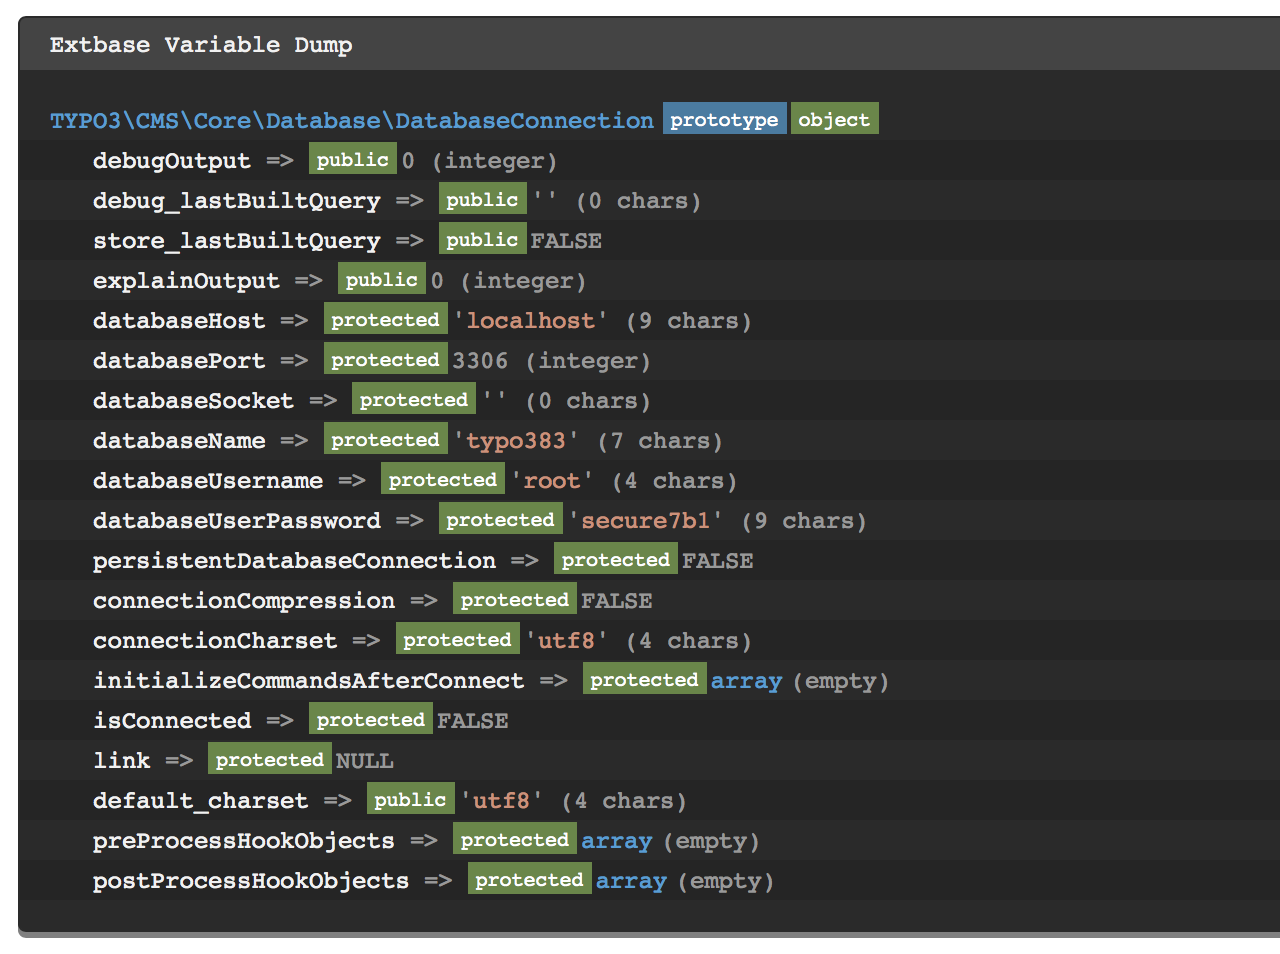
\includegraphics[width=0.65\linewidth]{InDepthChanges/76008.png}
	\end{figure}

\end{frame}

% ------------------------------------------------------------------------------
% LTXE-SLIDE-START
% LTXE-SLIDE-UID:		4d46a0d1-8fb9437d-8dfb2c08-3e04af77
% LTXE-SLIDE-ORIGIN:	2b74180d-e68ba0c2-8826a2cf-8498f977 English
% LTXE-SLIDE-TITLE:		!Breaking: #73461 - Import module disabled for non admin users
% LTXE-SLIDE-REFERENCE:	!Breaking-73461-ImportModuleDisabledForNonAdminUsers.rst
% ------------------------------------------------------------------------------
\begin{frame}[fragile]
	\frametitle{Korenite promene}
	\framesubtitle{Modul za uvoz je onemogucen za korisnike koji nisu administratori}

	\begin{itemize}

		\item Kao podrazumevano podesavanje, modul za uvoz \texttt{EXT:impexp} je sada onemogucen 
			za korisnike koji nisu administratori

		\item Za korisnike koji nisu administratori, a potrebna im je ova funkcionalnost, 
			ona se moze ukljuciti tako sto se User TSconfig opcija namesti:\newline
			\texttt{options.impexp.enableImportForNonAdminUser = 1}

			\vspace{0.5cm}

			\begingroup
				\color{typo3red}
				Upozorenje: ovo moze postati bezbednosni problem u TYPO3 verzijama 6.2 i 7.6
				i treba se omoguciti jedino korisnicima administratorskog interfejsa \textit{ od poverenja}.
			\endgroup

	\end{itemize}

\end{frame}

% ------------------------------------------------------------------------------
% LTXE-SLIDE-START
% LTXE-SLIDE-UID:		28772817-2c8fb763-8c2db24d-64180f1f
% LTXE-SLIDE-ORIGIN:	bac423cc-ba00db30-e1538b7f-25749380 English
% LTXE-SLIDE-TITLE:		Hooks and Signals (1)
% LTXE-SLIDE-REFERENCE:	!Feature-76209-HookToRegisterCustomResultBrowsersInAbstractPlugin.rst
% ------------------------------------------------------------------------------
\begin{frame}[fragile]
	\frametitle{Korenite promene}
	\framesubtitle{Hooks i Signals (1)}

	% decrease font size for code listing
	\lstset{basicstyle=\tiny\ttfamily}

	\begin{itemize}

		\item Novi hook omogucava implementaciju razlicitih resenja za razlicite pretrazivace

		\item Ovaj pristup omogucava da se pregazi podrazumevana implementacija
			\texttt{AbstractPlugin::pi\_list\_browseresults()}
			za sva prosirenja ili samo za odredjena

		\item Hook se moze registrovati u \texttt{ext\_localconf.php}:

			\begin{lstlisting}
				$GLOBALS['TYPO3_CONF_VARS']['SC_OPTIONS']
				  [\TYPO3\CMS\Frontend\Plugin\AbstractPlugin::class]['pi_list_browseresults'][1463475262] =
				  \Vendor\ExtensionKey\Hook\ResultBrowserHook::class
			\end{lstlisting}

	\end{itemize}

\end{frame}


% ------------------------------------------------------------------------------
% LTXE-SLIDE-START
% LTXE-SLIDE-UID:		a27998e5-f119c898-1dfacd18-06f1fb6f
% LTXE-SLIDE-ORIGIN:	82c70aee-3b375252-6cac0ad6-b385b95f English
% LTXE-SLIDE-TITLE:		Hooks and Signals (2)
% LTXE-SLIDE-REFERENCE:	!Feature-76259-IntroduceBuildQueryParametersPostProcessHook.rst
% ------------------------------------------------------------------------------
\begin{frame}[fragile]
	\frametitle{Korenite promene}
	\framesubtitle{Hooks i Signals (2)}

	% decrease font size for code listing
	\lstset{basicstyle=\tiny\ttfamily}

	\begin{itemize}

		\item Sa prelazom na Doctrine, hook \texttt{buildQueryParameters} je predstavljen u klasi
			\texttt{DatabaseRecordList}.

		\item Ovaj hook zamenjuje hook \texttt{makeQueryArray} iz zastarele metode
			\texttt{AbstractDatabaseRecordList::makeQueryArray}.

		\item Koriscenje novog hook-a dozvoljava izmenu parametara koji se koriste za upit u bazi podataka
			kako bi se dobili zapisi koji ce se prikazati u listi zapisa.

		\item Hook se moze registrovati u \texttt{ext\_localconf.php}:

			\begin{lstlisting}
				$GLOBALS['TYPO3_CONF_VARS']['SC_OPTIONS']
				  [\TYPO3\CMS\Recordlist\RecordList\DatabaseRecordList::class]['buildQueryParameters'][]
			\end{lstlisting}

		\item ...i implementira javnu metodu \texttt{buildQueryParametersPostProcess}

	\end{itemize}

\end{frame}

% ------------------------------------------------------------------------------
% LTXE-SLIDE-START
% LTXE-SLIDE-UID:		1bc35a6b-5ac0fd0c-3d8feb30-6b329f34
% LTXE-SLIDE-ORIGIN:	73d888ce-a14c0f6a-d4dec5fb-f7368bb6 English
% LTXE-SLIDE-TITLE:		!Breaking: #76108 - Replace ExtJS category tree with D3 and SVG
% LTXE-SLIDE-TITLE:		!Feature: #77349 - Additional locations for extension icons
% LTXE-SLIDE-TITLE:		!Feature: #77481 - Add possibility to define a favicon for the backend
% LTXE-SLIDE-REFERENCE:	!Breaking-76108-ReplaceExtJSCategoryTreeWithD3AndSVG.rst
% LTXE-SLIDE-REFERENCE:	!Feature-77349-AdditionalLocationsForExtensionIcons.rst
% LTXE-SLIDE-REFERENCE:	!Feature-77481-AddPossibilityToDefineAFaviconForTheBackend.rst
% ------------------------------------------------------------------------------
\begin{frame}[fragile]
	\frametitle{Korenite promene}
	\framesubtitle{Razno}

	\begin{itemize}

		\item SVG i D3 renderanje

			\begin{itemize}
				\item Kao deo uklanjanja ExtJS iz TYPO3 core-a, stablo unutar forme za izmenu je preradjeno
				\item Renderanje je sada bazirano na SVG i D3, sto donosi znacajno poboljsanje u preformansi
				\item Na isti nacin je planirana i prerada stabla strana u skoroj buducnosti
			\end{itemize}

		\item Ikonice prosirenja sada se mogu cuvati u sledecem direktorijumu:\newline
			\small
				\texttt{Resources/Public/Icons/<filename>}
				((gde <filename> moze biti: \texttt{Extension.png}, \texttt{Extension.svg} ili \texttt{Extension.gif})
			\normalsize

		\item Nova opcija \texttt{backendFavicon} u konfiguraciji Extension Manager-a 
			dozvoljava mogucnost promene favicon za administratorski interfejs.

	\end{itemize}

\end{frame}

% ------------------------------------------------------------------------------
